\documentclass[10pt,foldmark,notumble]{leaflet}

\usepackage[utf8]{inputenc}
\usepackage{graphicx}
\usepackage{listingsutf8}
\usepackage{color}
\usepackage[usenames,x11names]{xcolor}
\definecolor{citeGray}{HTML}{696969}
\definecolor{bulletlist}{HTML}{001020}
\definecolor{section}{HTML}{111111}
\definecolor{subsection}{HTML}{222222}
\definecolor{subsubsection}{HTML}{333333}
\usepackage{fourier}
\usepackage[top=0cm,bottom=0cm,left=0cm,right=0cm]{geometry}
\usepackage{caption}
\usepackage{makeidx}
\usepackage{amsmath,amsfonts,amssymb}
\usepackage{adjustbox}
\usepackage{blindtext}
\usepackage[babel=true]{csquotes}
\captionsetup{figurewithin=none}
\captionsetup{tablewithin=none}
\usepackage{changepage}

\def\changemargin#1#2#3#4{\list{}{\parsep#4\topsep#3\rightmargin#2\leftmargin#1}\item[]}
\let\endchangemargin=\endlist

\newcommand{\bmar}{\begin{changemargin}{0.2cm}{0.2cm}{-0.07cm}{0cm} }
\newcommand{\emar}{\end{changemargin}}

\lstset{literate=
  {á}{{\'a}}1 {é}{{\'e}}1 {í}{{\'i}}1 {ó}{{\'o}}1 {ú}{{\'u}}1
  {Á}{{\'A}}1 {É}{{\'E}}1 {Í}{{\'I}}1 {Ó}{{\'O}}1 {Ú}{{\'U}}1
  {à}{{\`a}}1 {è}{{\`e}}1 {ì}{{\`i}}1 {ò}{{\`o}}1 {ù}{{\`u}}1
  {À}{{\`A}}1 {È}{{\'E}}1 {Ì}{{\`I}}1 {Ò}{{\`O}}1 {Ù}{{\`U}}1
  {ä}{{\"a}}1 {ë}{{\"e}}1 {ï}{{\"i}}1 {ö}{{\"o}}1 {ü}{{\"u}}1
  {Ä}{{\"A}}1 {Ë}{{\"E}}1 {Ï}{{\"I}}1 {Ö}{{\"O}}1 {Ü}{{\"U}}1
  {â}{{\^a}}1 {ê}{{\^e}}1 {î}{{\^i}}1 {ô}{{\^o}}1 {û}{{\^u}}1
  {Â}{{\^A}}1 {Ê}{{\^E}}1 {Î}{{\^I}}1 {Ô}{{\^O}}1 {Û}{{\^U}}1
  {œ}{{\oe}}1 {Œ}{{\OE}}1 {æ}{{\ae}}1 {Æ}{{\AE}}1 {ß}{{\ss}}1
  {ç}{{\c c}}1 {Ç}{{\c C}}1 {ø}{{\o}}1 {å}{{\r a}}1 {Å}{{\r A}}1
  {€}{{\EUR}}1 {£}{{\pounds}}1
}

\usepackage{sectsty}
\sectionfont{\color{section}{}}
\subsectionfont{\color{subsection}{}}
\subsubsectionfont{\color{subsubsection}{}}
\definecolor{grisFonce}{HTML}{333333}
\definecolor{grisClair}{HTML}{dddddd}
\lstset{ %
  backgroundcolor=\color{grisClair},
  breaklines=true,
  language=[LaTeX]{TeX}
  }
\usepackage[colorlinks,urlcolor=grisFonce,linkcolor=grisFonce]{hyperref}
\usepackage{titlesec}
\titlespacing*{\section}
  {0.25cm}% decalage a gauche (positif ou negatif)
  {1ex}% espacement vertical avant
  {1ex}% espacement vertical apres
\titlespacing*{\subsection}
  {0.5cm}% decalage a gauche (positif ou negatif)
  {1ex}% espacement vertical avant
  {1ex}% espacement vertical apres
\titlespacing*{\subsubsection}
  {0.75cm}% decalage a gauche (positif ou negatif)
  {1ex}% espacement vertical avant
  {1ex}% espacement vertical apres



% modif 19 decembre 2003
\usepackage[francais]{babel}

%% modif du 25 novemebre 1999
%http://www.tug.dk/FontCatalogue/dejavusans/
%\usepackage[T1]{fontenc}
%\renewcommand*\familydefault{\sfdefault} %% Only if the base font of the document is to be sans serif
\usepackage[light]{kurier}
\usepackage[T1]{fontenc}

\setlength{\parindent}{0pt}
\setlength{\parskip}{0pt}

\title{\#Jaizappé ...}
\author{Servuc}
\date{2016}


\pdfinfo{%
  /Title    (\#Jaizappé ...)
  /Author   (Servuc)
  /Creator  (Servuc)
  /Producer (Servuc)
  /Subject  (Cours)
  /Keywords ()
}


\begin{document}
    \fcolorbox{black}{black}{
    \begin{minipage}{\linewidth}
        \begin{center}
            {\Huge{\color{white}\#Jaizappé ...\\... le C++ Arduino}}
        \end{center}
    \end{minipage}}
    \section{Histoire}
        L'Arduino, ou Genuino est une plateforme de prototypage basée sur un micro-controleur \textit{Atmel} en général.\\
        Il existe plusieurs boards avec chacune des spécificités.

        \emph{Ce mémo est inspiré de la documentation Arduino.}
    \section{Base}
        \subsection{Code de base}
        Le code d'un projet Arduino de base :

        \begin{lstlisting}[language=C]
void setup() {
    //Exécuté en premier
}
void loop() {
    //Exécuter après setup() en boucle
}
        \end{lstlisting}


        \subsection{Calcul binaire}
            Récupérer la partie \textit{big} et \textit{low} :

            \begin{lstlisting}[language=C]
highByte(value);
lowByte(value);
            \end{lstlisting}
            Lire, écrire les bits à partir de la droite, \textit{value} : valeur numérique
            \begin{lstlisting}[language=C]
bitRead(value, position);
bitWrite(value, position, bit); //bit = 0 ou 1
            \end{lstlisting}
            Quelques raccourcis (\textit{val}ue et \textit{pos}ition):

            \begin{lstlisting}[language=C]
bitSet(val, pos);   //bitWrite(val, pos, 1);
bitClear(val, pos); //bitWrite(val, pos, 0);
            \end{lstlisting}


        \subsection{Analyse des caractères}
            \begin{lstlisting}[language=C]
isAlphaNumeric(thisChar); // [a-zA-Z0-9]
isAlpha(thisChar);        // [a-zA-Z]
isAscii(thisChar);
isWhitespace(thisChar);
isControl(thisChar);      // \n \r ...
isDigit(thisChar);        // [0-9]
isLowerCase(thisChar);    // [a-z]
isUpperCase(thisChar);    // [A-Z]
isPrintable(thisChar);    // Affichable
isPunct(thisChar);
isHexadecimalDigit(thisChar);
            \end{lstlisting}

    \section{Débugage et série}
        \subsection{Serial}
            Initialisation (une seule fois !) :
            \begin{lstlisting}[language=C]
Serial.begin( SPEED );
            \end{lstlisting}
            \textbf{SPEED} vaut $9600$, $57600$ ou $115200$ en général. Vitesse en baud.\\
            Écrire le moniteur de débug :
            \begin{lstlisting}[language=C]
Serial.print( VARIABLE );   //Pas de \n
Serial.println( VARIABLE ); //Avec \n
            \end{lstlisting}

            Dans le cas d'un \textit{float} :
            \begin{lstlisting}[language=C]
Serial.print( VARIABLE, precision );
            \end{lstlisting}

            Lire ce qui est sur le port série (byte par byte), utiliser dans \textit{loop()} :
            \begin{lstlisting}[language=C]
if (Serial.available() > 0) {
    byte incomingByte = Serial.read();
}
            \end{lstlisting}
        \subsection{SoftwareSerial}
            Fonctionne comme \textit{Serial}. Nécessite :
            \begin{lstlisting}[language=C]
#include <SoftwareSerial.h>
            \end{lstlisting}
            Initialisation (inutile pour \textit{Serial}) :
            \begin{lstlisting}[language=C]
SoftwareSerial mSerial(PIN_RX, PIN_TX);
            \end{lstlisting}
            \textbf{IMPORTANT !} Pour communiquer entre 2 supports :
            \begin{itemize}
                \item Support 1 : \textit{RX} $\leftrightarrow$ \textit{TX} : Support 2
                \item Support 1 : \textit{TX} $\leftrightarrow$ \textit{RX} : Support 2
            \end{itemize}
            Si \textit{SoftwareSerial} sont initialisés, un seul peut être en écoute :
            \begin{lstlisting}[language=C]
mSerial.listen();
mSerial.isListening();
            \end{lstlisting}

    \section{Les Pins}
        Il est conseillé de définir les pins :
        \begin{lstlisting}[language=C]
#define PIN_FCT_ABCD 5
        \end{lstlisting}

        Indiquer le mode le pin (dans \textit{setup()}):

        \begin{lstlisting}[language=C]
pinMode( PIN_ID, INPUT );  //Lecture
pinMode( PIN_ID, OUTPUT ); //Ecriture
        \end{lstlisting}

        \subsection{Analogiques}
            Notées $AX$ ($X$ un nombre). \textbf{PIN\_ID} noté $AX$ aussi.\\
            Mettre la valeur d'un pin (mode \textbf{OUTPUT}) :

            \begin{lstlisting}[language=C]
analogWrite( PIN_ID, value ); // 0 - 255
            \end{lstlisting}
            \vspace{0.5cm}
            Récupérer la valeur d'un pin (pas de mode):

            \begin{lstlisting}[language=C]
int myVal = analogRead( PIN_ID );
float myVoltage = myVal * (VOLT_MAX / 1023.0);
            \end{lstlisting}

            Fixé la valeur de lecture sur les pins analogiques :

            \begin{lstlisting}[language=C]
analogReference(value);
            \end{lstlisting}
            \begin{center}
                \begin{tabular}{| l | l | l |}
                    \hline
                        Arduino & \textit{value} & Description \\
                    \hline
                        Tous & \textbf{DEFAULT} & $5V$ ou $3.3V$ \\
                        ATMega 168/328 & \textbf{INTERNAL} & $1.1V$ \\
                        ATMega 8 & \textbf{INTERNAL} & $2.56V$ \\
                        Ard. Mega & \textbf{INTERNAL1V1} & $1.1V$ \\
                        Ard. Mega & \textbf{INTERNAL2V56} & $2.56V$ \\
                        Tous & \textbf{EXTERNAL} & Sur \textit{AREF} ($0V$ - $5V$) \\
                    \hline
                \end{tabular}
            \end{center}

        \subsection{Digitals}

            Notées $dX$ ou $X$ ($X$ un nombre). Égale à $0$ ou $1$.\\
            Correspondant respectivement à \textbf{LOW} et \textbf{HIGH}.\\

            Mettre la valeur d'un pin (mode \textbf{OUTPUT}) :

            \begin{lstlisting}[language=C]
digitalWrite( PIN_ID, HIGH ); //1 = 5V ou 3.3V
digitalWrite( PIN_ID, LOW );  //0 = 0V
            \end{lstlisting}

            Récupérer la valeur d'un pin (mode \textbf{INPUT}) :

            \begin{lstlisting}[language=C]
int myVal = digitalRead( PIN_ID );
            \end{lstlisting}

            Cependant, il faut stabiliser le pin à 0 ou 5/3.3V. Exemple :

            \begin{center}
                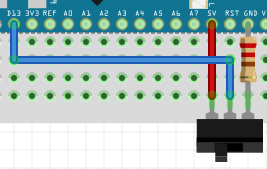
\includegraphics[scale=0.5]{img/arduino-1}
            \end{center}


        \subsection{Usage avancé}
            Inutilisable avec les Arduino \textit{Gemma} et \textit{Due}.\\
            Émettre une tonalité avec un Arduino avec un piezo, un haut parleur,
            \textbf{pin} doit être noté \textit{PWM}. \textbf{time} en millisecondes.

            \begin{center}
                 \begin{tabular}{| l | l | l |}
                    \hline
                        Arduino & Fréq. min & Fréq. max \\
                    \hline
                        Tous & $31$ & $65535$ \\
                        Zero & $41$ & $275000$ \\
                    \hline
                \end{tabular}
            \end{center}
            \begin{lstlisting}[language=C]
tone( pin, frequency );      //Ou
tone( pin, frequency, time );
            \end{lstlisting}

            Pour arrêter la première instruction :
            \begin{lstlisting}[language=C]
noTone();
            \end{lstlisting}


            Lire une impulsion (signal continu)sur un pin digital de 10 microsecondes à 3 minutes,\\
            \textit{value} : \textbf{HIGH} et \textbf{LOW}, \textit{timeout} : Attente max. en microsecondes.
            \begin{lstlisting}[language=C]
pulseIn( pin, value );
pulseIn( pin, value, timeout );
            \end{lstlisting}

    \section{Veille et interruptions}
        Pour mettre un Arduino :
        \begin{lstlisting}[language=C]
delay( MILLI_SECONDS );
delayMicroseconds( MICRO_SECONDS );
        \end{lstlisting}
        Un \textit{delay()} peut être arrêté par une interaction sur un pin digital :

        \begin{center}
            \begin{tabular}{| l | l |}
                \hline
                    Uno, Nano, base 328 & $2, 3$\\
                \hline
                    Mega, Mega2560, MegaADK & $2, 3, 18, 19, 20, 21$\\
                \hline
                    Micro, Leonardo, base 32u4 & $0, 1, 2, 3, 7$\\
                \hline
                    Zero & Toutes sauf la $4$\\
                \hline
                    MKR1000 Rev.1 & $0, 1, 4, 5, 6, 7, 8, 9, A1, A2$\\
                \hline
                    Due, 101 & Toutes\\
                \hline
            \end{tabular}
        \end{center}

        Attacher une fonction à l'interruption :
        \begin{lstlisting}[language=C]
attachInterrupt(
    digitalPinToInterrupt( PIN_ID ),
    FUNCTION , MODE);
        \end{lstlisting}

        \begin{enumerate}
            \item \textbf{FUNCTION} : Une fonction de type \textit{void} sans paramètre;
            \item \textbf{MODE} :
            \begin{enumerate}
                \item \textbf{LOW} : Si le pin est à 0 (\textbf{LOW});
                \item \textbf{CHANGE} : Tension qui change;
                \item \textbf{RISING} : \textbf{LOW} à \textbf{HIGH};
                \item \textbf{FALLING} : \textbf{HIGH} à \textbf{LOW};
                \item \textbf{HIGH} : Pin à 1 (Sur \textit{Due}, \textit{Zero} et \textit{MKR1000}).
            \end{enumerate}
        \end{enumerate}

        Enlever une interruption sur un pin :
        \begin{lstlisting}[language=C]
detachInterrupt(
    digitalPinToInterrupt( PIN_ID ));
        \end{lstlisting}

        \textbf{IMPORTANT} : Les variables partagées doivent être \textit{volatile} :

        \begin{lstlisting}[language=C]
volatile int mCount = 0;
void buttonPressed () { //Fct interrup.
    mCount++;
}
void loop() {
    Serial.println(mCount); delay(7331);
}
        \end{lstlisting}

        Mettre en pause les interruptions pour les codes critiques :
        \begin{lstlisting}[language=C]
noInterrupts();
    //Code that MUST be not interrupt
interrupts();
        \end{lstlisting}
    \section{Mathématiques et temps}
        \subsection{Général}
            \begin{center}
                \begin{tabular}{l l | l l | l l}
                    Sinus & $sin(x,y)$ & Cosinus & $cos(x) $ & Tang. & $tan(x,y)$\\
                    Mini. & $min(x,y)$ & Racine & $sqrt(x) $ & Absolu & $abs(x,y)$\\
                    Maxi. & $max(x,y)$ & Puiss. & $pow(x,y)$ & &\\ \\
                \end{tabular}
            \end{center}

            $constrain(x, min, max)$ : Retourne $x$ si $min < x < max$ sinon une valeur extrème.\\
            $map(x, minSource, maxSource, minDest, maxDest)$ : Retourne $x$ adapté aux extrèmes de destination en fonction des extrèmes sources.

        \subsection{Aléatoire}
            Changer la \textit{seed} de l'aléatoire :
            \begin{lstlisting}[language=C]
randomSeed(analogRead(0));
randomSeed(numberValue);
            \end{lstlisting}

            Avoir un nombre aléatoire,
            \textit{min} inclusif, \textit{max} exclusif
            \begin{lstlisting}[language=C]
long random(max);
long random(min, max);
            \end{lstlisting}

        \subsection{Temps}
            Temps écoulé depuis le démarrage :
            \begin{lstlisting}[language=C]
unsigned long millis();
unsigned long micros();
            \end{lstlisting}
            \textit{Overflow} de \textit{millis()} et \textit{micros()} à $50$ jours et $70$ minutes.\\
            Faire patienter quelques instants :
            \begin{lstlisting}[language=C]
delay(milliSeconds);
delayMicroseconds(microSeconds);
            \end{lstlisting}


    \section{Mémoire}
        \subsection{EEPROM}
            Un Arduino a une mémoire flash pour les variables, l'EEPROM.\\
            Attention, le nombre d'écriture est limitée !
            \begin{lstlisting}[language=C]
#include <EEPROM.h>
            \end{lstlisting}
            Vider l'EEPROM :
            \begin{lstlisting}[language=C]
for (int i = 0 ; i < EEPROM.length() ; i++) {
    EEPROM.write(i, 0);
}
            \end{lstlisting}
            Écrire dans l'EEPROM :
            \begin{lstlisting}[language=C]
EEPROM.write(address, value); // 0-255
EEPROM.put(address, value);   // all
            \end{lstlisting}
            Lire dans l'EEPROM, le \textit{get()} ne nécessiste pas de cast :
            \begin{lstlisting}[language=C]
byte value1;  MyObject value2;
EEPROM.read(address, value1); // 0-255
EEPROM.get(address, value2);  // all
            \end{lstlisting}
            Mettre à jour une valeur que si besoin :
            \begin{lstlisting}[language=C]
EEPROM.update(address, value); // 0-255
            \end{lstlisting}

        \subsection{Autres}
            S'il manque de la mémoire pour une chaine de caractères, la macro \textit{F(string)} permet de la stocker dans la flash :
            \begin{lstlisting}[language=C]
Serial.print(F("Very long string"));
            \end{lstlisting}
            Taille d'une variable, un type, un tableau en bytes :
            \begin{lstlisting}[language=C]
sizeof(int); int a = 1; sizeof(a);
            \end{lstlisting}
            Stocker dans la flash, à la place de la SRAM :\\
            Suivant le compilateur, une des deux versions fonctionnent !
            \begin{lstlisting}[language=C]
#include <avr/pgmspace.h>
const type varName[] PROGMEM = {d0, d1, ...};
const PROGMEM type varName[] = {d0, d1, ...};
            \end{lstlisting}



            \begin{center}
                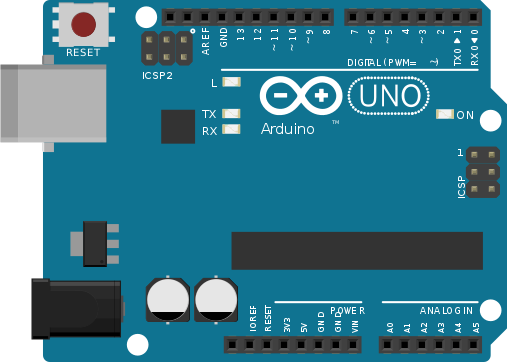
\includegraphics[scale=0.6]{img/arduino-uno-frietzing}
            \end{center}
    \vfill
\fcolorbox{black}{black}{
\begin{minipage}{\linewidth}
{\color{white}\begin{center}\hfill http://github.com/Servuc/jaizappe \hfill\LaTeX\hfill Licence GPLv3\hfill $\,$\end{center}}
\end{minipage}}
\end{document}